\newpage
\section{Auswertung}

    \subsection{Untersuchung von Quarzkügelchen}
        \subsubsection{Kamerakalibrierung}
        \label{sec:Pixel}
            Das in Abbildung \ref{fig:cal_cam} per optische Pinzette eingefangene Quarzkügelchen wird genutzt, um das Zentrum der optischen Falle (gelber Kreis) in der Kamersoftware zu markieren. Über den
            rot eingezeichneten Durchmesser von 65 Pixeln wird mithilfe des mittleren Durchmessers $\overline{\text{d}}$ eines Quarzkügelchens von \SI{2.06}{\micro\metre} eine Pixelgröße im Realraum von 
            %
            \begin{equation*}
                1\,\text{px} = \frac{\SI{2.06}{\micro\metre}}{65\pm4} \approx \SI{0.0317 +- 0.0020}{\micro\metre}
            \end{equation*}
            %
            berechnet. Der Fehler von 4 Pixeln wird aufgrund der visuellen Bestimmung des Randes des Quarzkügelchens angenommen.
            %
            \begin{figure}[h]
            \centering
            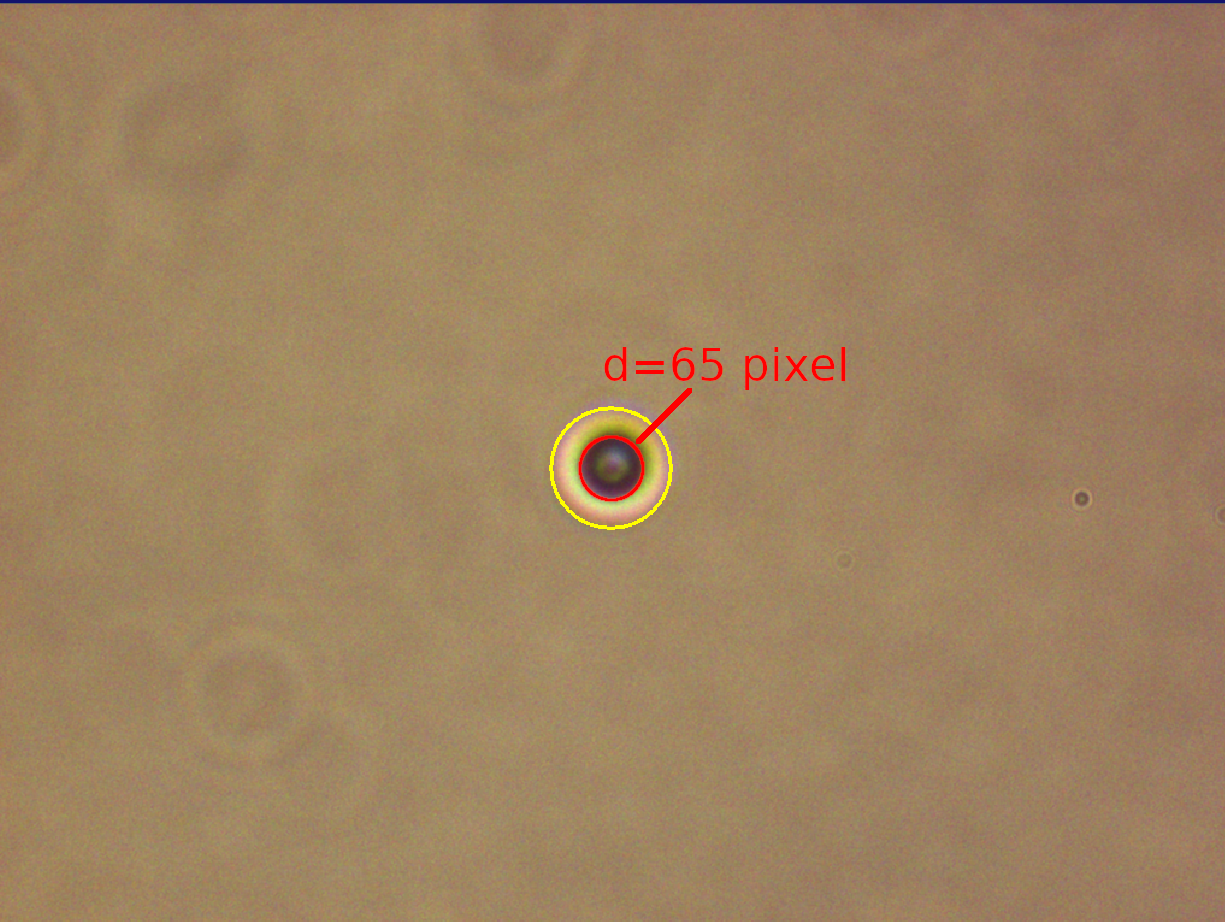
\includegraphics[width = 0.75\textwidth]{pictures/cal_cam.png}
            \caption{Abbildung eines in der optischen Falle (gelber Kreis) eingefangenen Quarzkügelchens (roter Kreis).}
            \label{fig:cal_cam}
            \end{figure}
            \FloatBarrier
            %

        \newpage
        \subsubsection{Kalibrierung der Photodiode}
            Die zur Kalibrierung der Photodiode aufgenommenen S-Kurven sind exemplarisch für eine Laserleistung von \SI{4.83}{\milli\watt} in einem Screenshot des Programms \ref{fig:pos_cal} für die x- und 
            y-Achse dargestellt. In diesem Screenshot sind auch die per Programm berechneten und in Grafik \ref{fig:Konversion} gegen die Laserleistung aufgetragenen Konversionsfaktoren der beiden Achsen 
            eingetragen.
            \FloatBarrier
            %
            \begin{figure}[h]
            \centering
            \includegraphics[width = 0.9\textwidth]{OP_Sternikov/Pos_Cal_50mA.png}
            \caption{Abbildung einer aufgenommenen S-Kurve bei einer Laserleistung von \SI{4.83}{\milli\watt} zur Kalibrierung der Konversionsfaktoren.}
            \label{fig:pos_cal}
            \end{figure}
            \FloatBarrier
            %         
            \newpage
            Daraus ergeben sich die Mittelwerte der Konversionsfaktoren
            \begin{equation*}
                \overline{K_{\text{x}}} = \SI{0.41115 +- 0.00033}{\volt\per\micro\metre} \qquad\qquad \overline{K_{\text{y}}} = \SI{0.26508 +- 0.00010}{\volt\per\micro\metre} \,,
            \end{equation*}
            die zur Berechnung der Position eines eingefangenen Objekts durch die von der Vier-Segment-Diode gemessenen Spannung benötigt werden.

            %
            \begin{figure}[h]
            \centering
            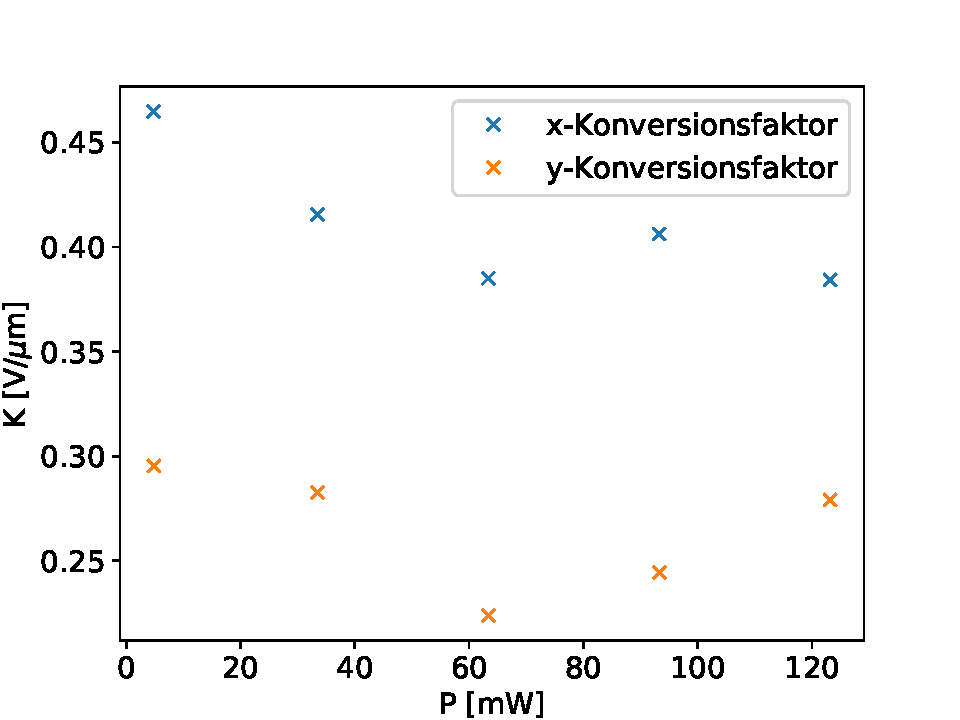
\includegraphics[width = 0.9\textwidth]{Konversion.pdf}
            \caption{Die für beide Achsen gemessenen Konversionsfaktoren bei unterschiedlichen Laserleistungen sowie deren Fehler, die zur Sichtbarkeit um den Faktor 10 vergrößert sind.}
            \label{fig:Konversion}
            \end{figure}
            \FloatBarrier
            %
            \newpage
            Das in Abhängigkeit des z-Piezo-Werts aufgenommene Diodensummensignal bei einem festen Quarzkügelchen ist in Abbildung \ref{fig:Diodensumme} aufgetragen. Der Verlauf der Kurve entspricht dem zu erwartenden Anstieg in der Umgebung des Streumaximus und bestätigt, dass ein festes Quarzkügelchen vermessen wurde.
            %
            \begin{figure}[h]
            \centering
            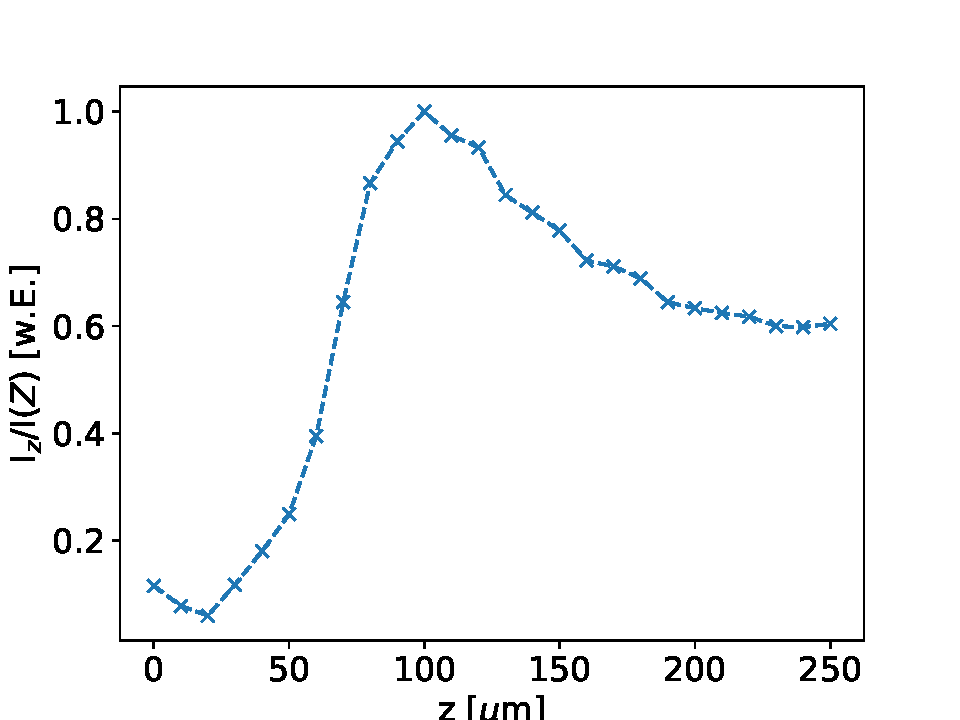
\includegraphics[width = 0.75\textwidth]{Diodensumme.pdf}
            \caption{Das gemessene Diodensummensignal gegen die z-Position der optischen Falle im Bereich um das Streumaximum hier bei circa \SI{100}{\micro\metre}.}
            \label{fig:Diodensumme}
            \end{figure}
            \FloatBarrier
            %


        \newpage
        \subsubsection{Kalibrierung der Fallensteifigkeit}
            Der letzte Schritt der Kalibrierung, umfasst die Bestimmung der Fallensteifigkeiten $k_x$ und $k_y$ für beide Achsen.
            
            Für die Kalibrierung ohne externe Krafteinwirkung wird die spektrale Leistungsdichte (PSD) genutzt, die im Screenshot \ref{fig:PSD} für beide Achsen bei einer Laserleistung von 
            \SI{63.4}{\milli\ampere} dargestellt ist und direkt aus dem Programm exportiert werden kann. 
            %
            \begin{figure}[h]
            \centering
            \includegraphics[width = 0.75\textwidth]{OP_Sternikov/k_noForce_150mA.png}
            \caption{Bildschirmaufnahme des Programms zur Messung der Fallensteifigkeit mit Abbildungen im Frequenzraum und den vom Programm berechneten Fallensteifigkeiten für beide Achsen.}
            \label{fig:PSD}
            \end{figure}
            \FloatBarrier
            %
            An diese Kurve wird folgende Funktion angepasst
            \begin{equation*}
                \text{PSD}(f) = \text{const} \cdot \frac{1}{f^2+f_0^2} \, ,
            \end{equation*}
            die die Frequenz $f$ sowie die sogenannte Roll-Off-Frequenz $f_0$ beinhaltet und die Eigenschaften der spektralen Leistungsdichte \ref{eqn:Leistung} wiedergibt. Aus diesen in Grafik 
            \ref{fig:freq_noForce} exemplarisch für eine Laserleistung von \SI{63.4}{\milli\ampere} dargestellten Anpassungen, werden die Fallensteifigkeiten über Formel \ref{eqn:Roll} und die in Tabelle
            \ref{tab:f_0} aufgelisteten Roll-Off-Frequenzen ausgerechnet und in Tabelle \ref{tab:noForce} aufgetragen. Da der erste und letzte Wert deutlich vom zu erwartenden ansteigenden Trend der drei 
            mittleren Werte abweichen, wird nur durch diese drei mittleren Werte eine lineare Ausgleichsgerade zur Kalibrierung der Fallensteifigkeit in Abhängigkeit der Laserleistung gelegt. Auch wenn 
            die Fallensteifigkeit vom Gradienten der Leistung senkrecht zur Strahlachse abhängt und dieser nicht linear verläuft, ist nach Masaaki Yasuda et al. \cite{yasuda_direct_2017} die Annahme einer
            linearen Abhängigkeit gerechtfertigt.  
            Dies ergibt folgende Kalibrierung in Abhängigkeit der Laserleistung in \si{\milli\watt} für den Bereich 
            von \SI{93.3}{\milli\watt} bis \SI{153.1}{\milli\watt}:
            \begin{align}
                k_x(\text{P}) &= 1.34\cdot10^{-8}\si{\newton\per\metre\milli\watt} \cdot \text{P} - 7.71\cdot10^{-7}\si{\newton\per\metre} \\
                k_y(\text{P}) &= 2.14\cdot10^{-8}\si{\newton\per\metre\milli\watt} \cdot \text{P} - 1.46\cdot10^{-6}\si{\newton\per\metre}
            \end{align}
            %
            \begin{figure}[h]
            \centering
            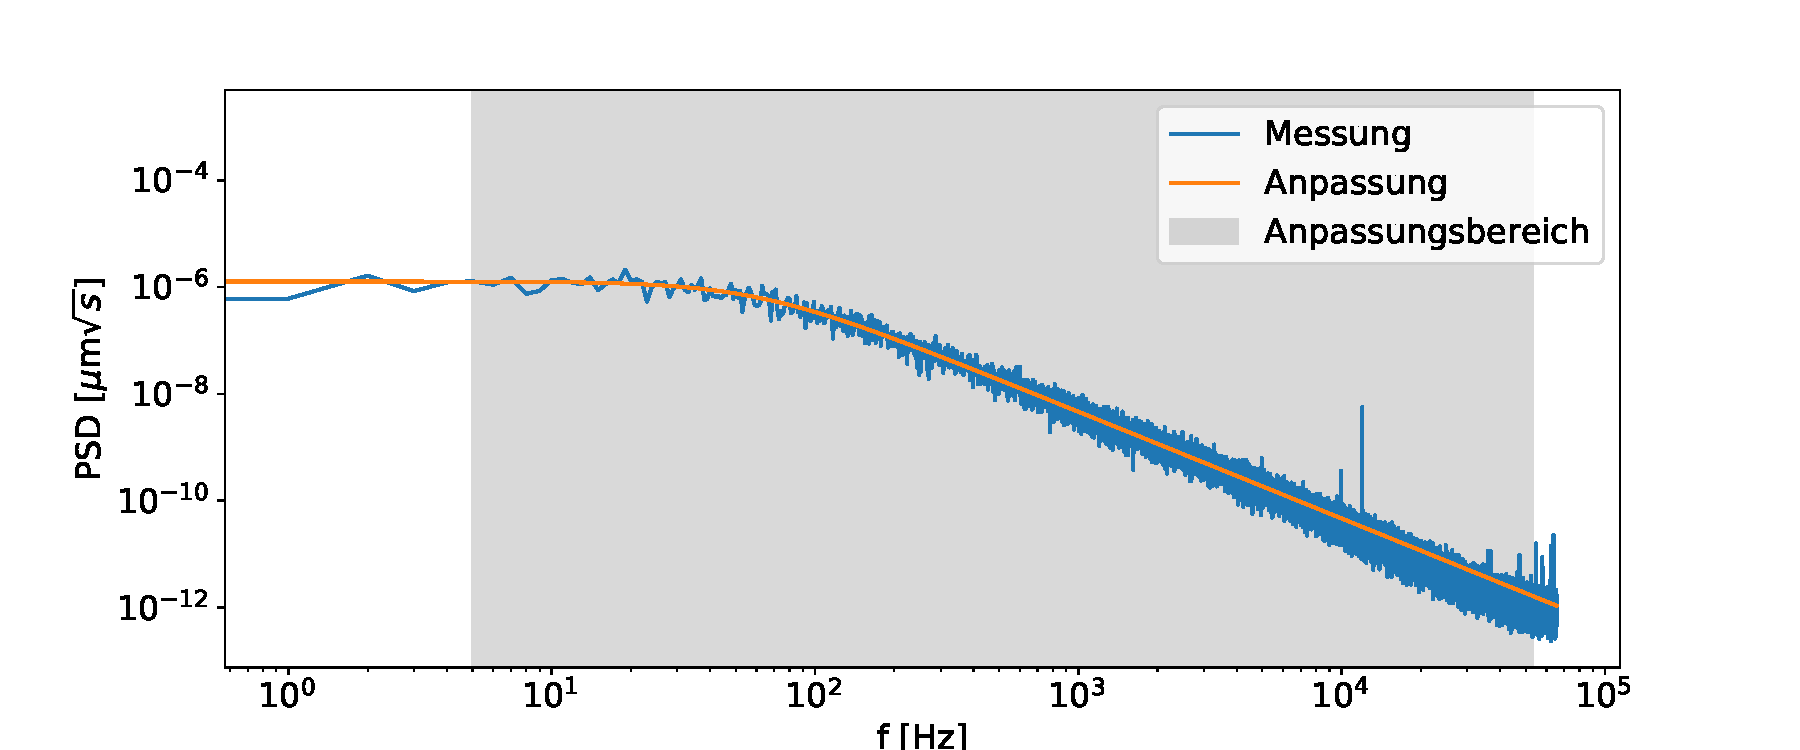
\includegraphics[width = 0.9\textwidth]{freq_x.pdf}
            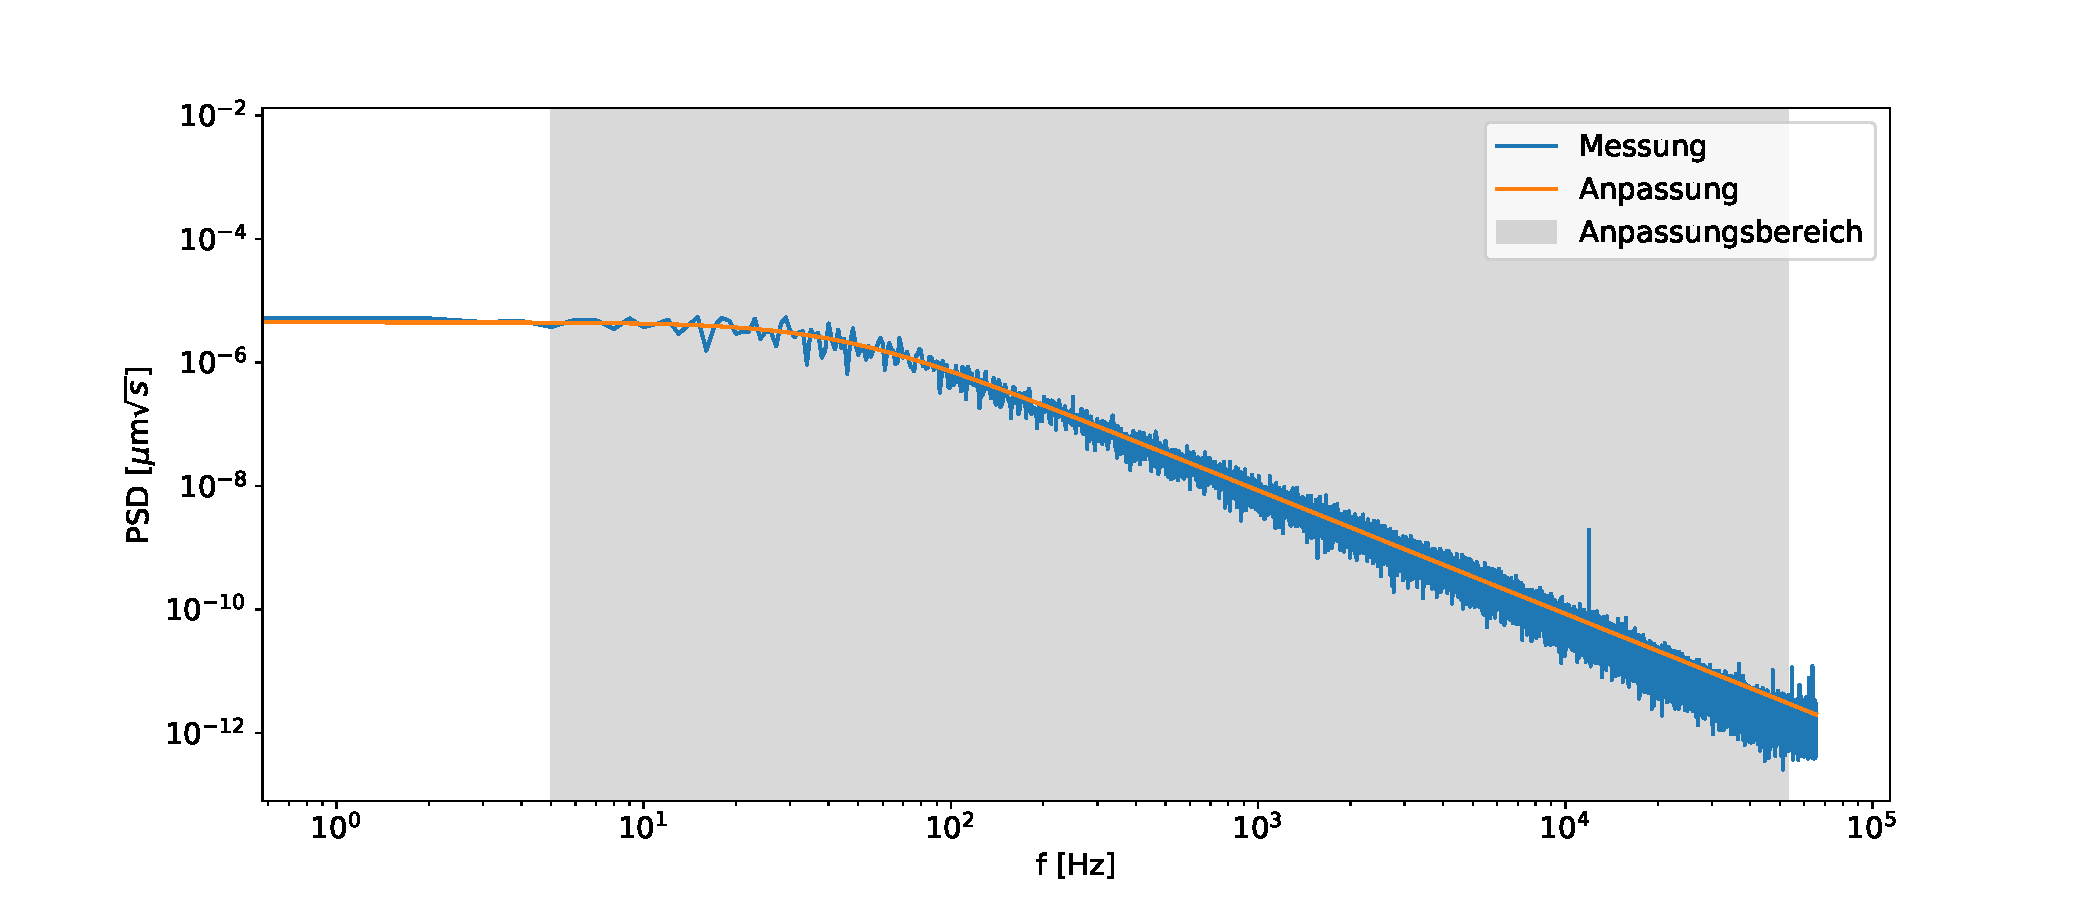
\includegraphics[width = 0.9\textwidth]{freq_y.pdf}
            \caption{Die spektrale Leistungsdichte oben für die x-Achse und unten für die y-Achse gegen die Frequenz aufgetragen sowie eine theoretische Anpassung, die auf den Werten im markierten Bereich beruht.}
            \label{fig:freq_noForce}
            \end{figure}
            \FloatBarrier
            % 
            %
            \begin{figure}[h]
            \centering
            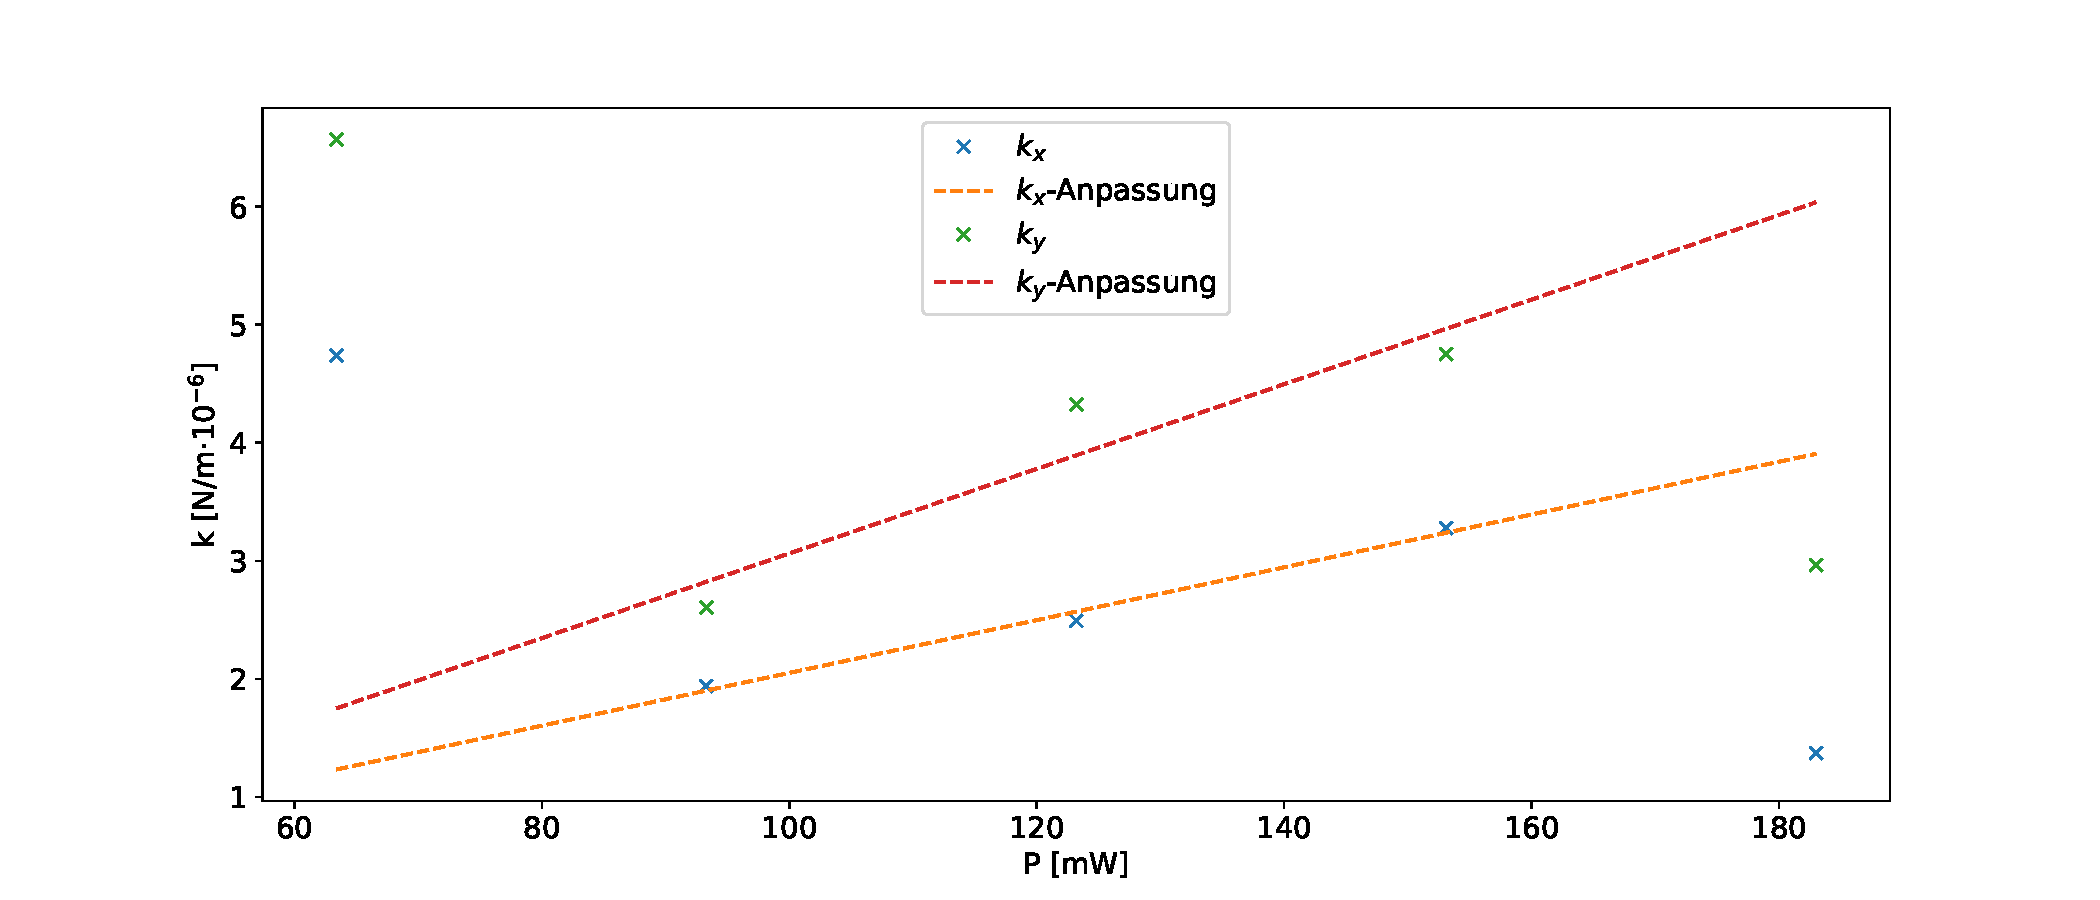
\includegraphics[width = 0.75\textwidth]{k_noForce.pdf}
            \caption{Aus den PSD-Anpassungen gewonnenen Fallensteifigkeiten aufgetragen gegen die Laserleistung und eine lineare Anpassung der mittleren drei Werte zur Kalibrierung der Fallensteifigkeiten.}
            \label{fig:k_noForce}
            \end{figure}
            \FloatBarrier
            %
            Zur Überprüfung der Kalibrierung wird aus der Variation der Position des Kügelchens aufgrund der Brown´schen Bewegung, die in den Grafiken \ref{fig:pos_noForce} für eine Laserleistung von 
            \SI{63.4}{\milli\watt}
            dargestellt ist, und den zuvor berechneten Fallensteifigkeiten die Boltzmannkonstante zu den in Tabelle \ref{tab:noForce} aufgelisteten Werten bestimmt.
            %
                        %
            \begin{table}[h]
                \centering
                \caption{Die aus den Anpassungen der PSD gewonnenen Roll-Off-Frequenzen bei verschiedenen Laserleistungen und keiner externen Krafteinwirkung.}
                \label{tab:f_0}
                \begin{tabular}{c c c}
                \toprule
                {P[mW]} &   {$f_{0\text{,x}}$ [Hz]} & {$f_{0\text{,y}}$ [Hz]}  \\
                \midrule
                \num{63.4}     &   \num{43.59 +- 0.12}	 &  \num{60.42 +- 0.15}  \\
                \num{93.3}     &   \num{17.85 +- 0.04}	 &  \num{23.99 +- 0.07}  \\
                \num{123.2}    &   \num{22.94 +- 0.06}	 &  \num{39.80 +- 0.11}  \\
                \num{153.1}    &   \num{30.15 +- 0.10}	 &  \num{43.70 +- 0.15}  \\
                \num{182.0}    &   \num{12.61 +- 0.03}	 &  \num{27.28 +- 0.10}  \\
                \bottomrule
                \end{tabular}
            \end{table}
            %
            \begin{table}[h]
                \centering
                \caption{Die über die aus der Anpassung der spektralen Leistungsdichte gewonnenen Roll-Off-Frequenzen berechneten Fallensteifigkeiten in x- und y-Richtung sowie die daraus berechneten Werte für die Boltzmannkonstante bei verschiedenen Laserleistungen und keiner externen Krafteinwirkung.}
                \label{tab:noForce}
                \begin{tabular}{c c c c c}
                \toprule
                {P[mW]} &   {$k_\text{x}$ [N/m]} & {$k_\text{B,x}$ [J/K]} &{$k_\text{y}$ [N/m]} & {$k_\text{B,y}$ [J/K]}  \\
                \midrule
                \num{63.4}     &   \num{4.737(13)e-6}	 &  \num{1.432(4)e-23}   &  \num{6.567(17)e-6}    &  \num{1.908(5)e-23}  \\
                \num{93.3}     &   \num{1.941(5)e-6}	 &  \num{7.751(19)e-24}   &  \num{2.607(8)e-6}    &  \num{1.561(5)e-23}  \\
                \num{123.2}    &   \num{2.493(6)e-6}	 &  \num{7.819(19)e-24}   &  \num{4.325(12)e-6}    &  \num{1.916(5)e-23}  \\
                \num{153.1}    &   \num{3.277(11)e-6}	 &  \num{8.253(28)e-24}   &  \num{4.749(16)e-6}    &  \num{1.735(6)e-23}  \\
                \num{182.0}    &   \num{1.370(3)e-6}	 &  \num{6.688(16)e-24}   &  \num{2.965(10)e-6}    &  \num{1.071(4)e-23}  \\
                \bottomrule
                \end{tabular}
            \end{table}
            %
            %
            \begin{figure}[h]
            \centering
            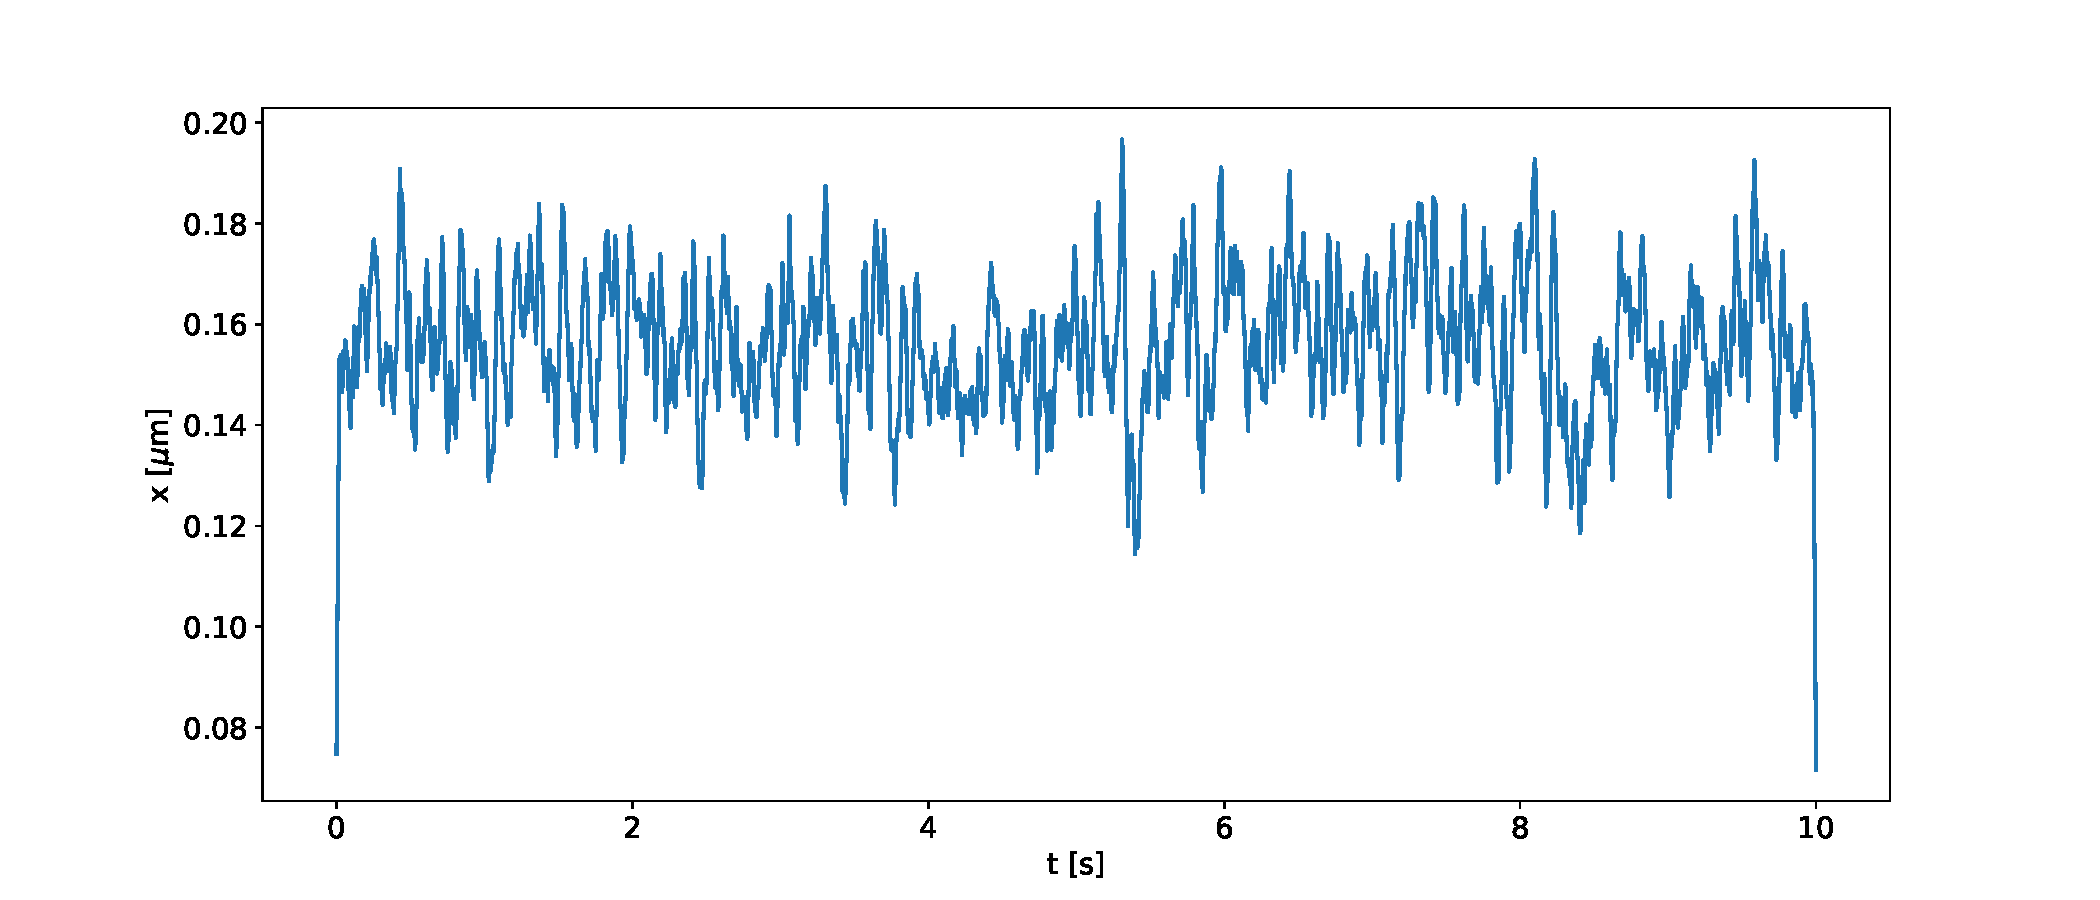
\includegraphics[width = 0.7\textwidth]{force_x.pdf}
            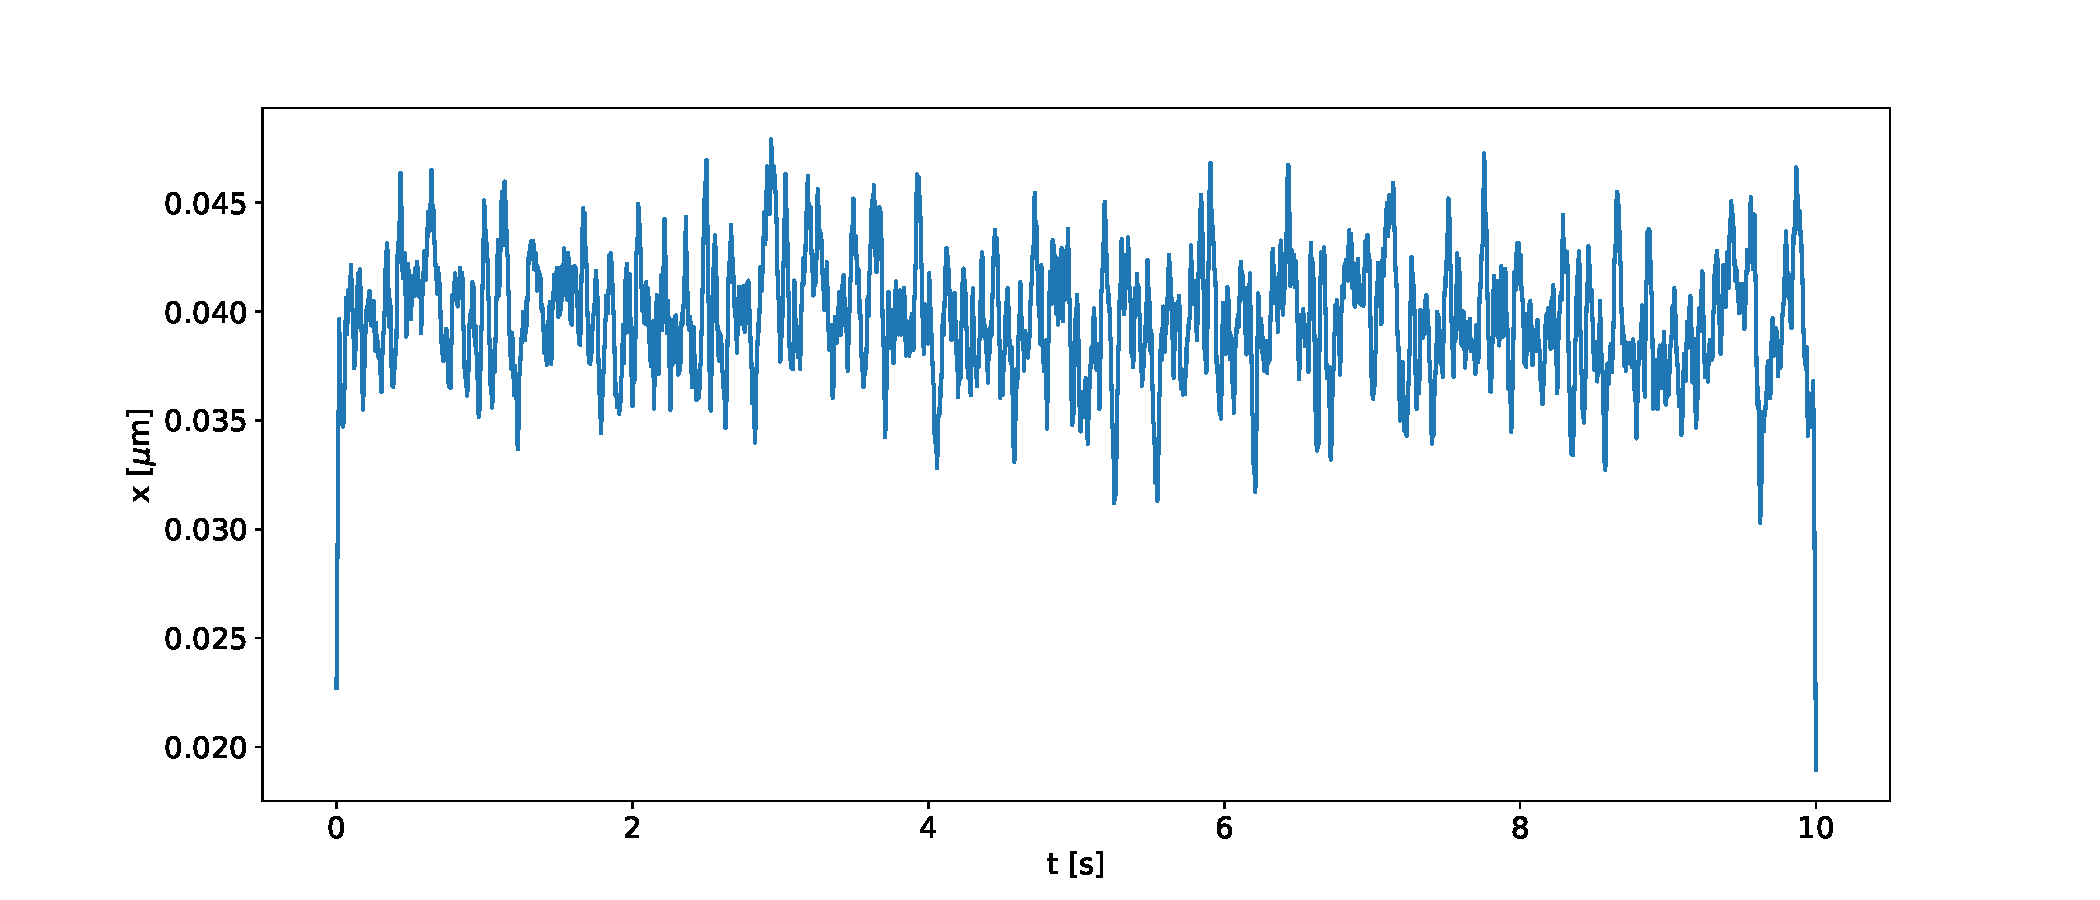
\includegraphics[width = 0.7\textwidth]{force_y.pdf}
            \caption{Der Ort des Quarzkügelchens aufgetragen gegen die Messzeit.}
            \label{fig:pos_noForce}
            \end{figure}
            \FloatBarrier
            % 

            
            % Bei Anregung mit einer externen Kraft kann die Bewegung des Quarzkügelchens als sinusförmige Schwingung
            % \begin{equation*}
            %     x(t) = \text{A} \sin\left(2\pift\right)
            % \end{equation*}
            % mit der Amplitude A und der Frequenz $f$ beschrieben werden. So lässt sich die wirkende Kraft mit Hilfe der Fallensteifigkeit $k_{x/y}$ berechnen. Wenn das Quarzkügelchens die optische Pinzette 
            % aufgrund der externen Kraft verlässt, kann die dort wirkende Kraft mit dem zuvor beschriebenen Weg zur Kraftberechnung gleichgesetzt werden. Es ergibt sich folgende Gleichung
            % \begin{equation*}
            %     da
            % \end{equation*} 

            Bei der Messung mit externer Krafteinwirkung und der Messung mit externer Krafteinwirkung sowie eingesetztem Vortex-Retarder werden die Messungen direkt vom Programm ausgewertet.
            Mit dessen gespeicherter Kalibrierung der S-Kurven, kann es die Fallensteifigkeiten berechnen und auslesen lassen. Da das Programm die Fallensteifigkeiten nicht fehlerbehaftet ausgibt, werden die 
            Fehler konservativ über die maximalen Fehler der Fallensteifigkeiten bei selbst durchgeführter Berechnung abgeschätzt. Diese nun fehlerbehafteten Werte sind für die Messung mit
            externer Krafteinwirkung in x-Richtung in Grafik \ref{fig:k_xForce} gegen die Laserleistung aufgetragen, wobei kein Zusammenhang zwischen den Werten der Fallensteifigkeiten und der Laserleistung 
            zu erkennen ist. Wie zuvor wird die Boltzmannkonstante über das Äquipartitionstheorem berechnet und mit den Fallensteifigkeiten in Tabelle \ref{tab:xForce} für die x-Richtung und in Tabelle 
            \ref{tab:yForce} für die y-Richtung aufgelistet. 
            %
            \begin{figure}[h]
            \centering
            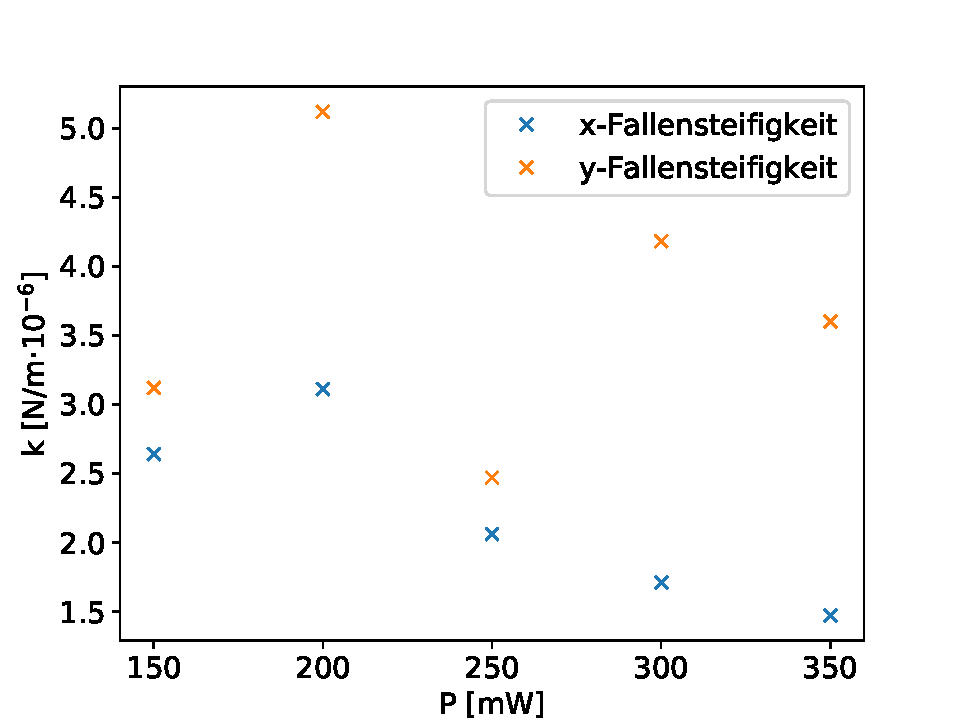
\includegraphics[width = 0.75\textwidth]{k_xForce.pdf}
            \caption{Vom Programm aus den PSD bestimmten Fallensteifigkeiten aufgetragen gegen die Laserleistung bei externer Krafteinwirkung in x-Richtung.}
            \label{fig:k_xForce}
            \end{figure}
            \FloatBarrier
            %
            %
            \begin{table}[h]
                \centering
                \caption{Die vom Programm über die spektralen Leistungsdichten berechneten Fallensteifigkeiten in x-Richtung sowie die daraus berechneten Werte für die Boltzmannkonstante bei verschiedenen Laserleistungen und externe Krafteinwirkung in x-Richtung.}
                \label{tab:xForce}
                \begin{tabular}{c c c c}
                \toprule
                {P[mW]} &   {$\langle\text{x}^2\rangle$ [\si{\square\micro\metre}]} &  {$k_\text{x}$ [N/m]} & {$k_\text{B,x}$ [J/K]} \\
                \midrule
                \num{63.4}     &   \num{1.61e-3}    &   \num{2.640(20)e-6}	 &  \num{1.422(11)e-23}    \\
                \num{93.3}     &   \num{1.08e-3}    &   \num{3.110(20)e-6}	 &  \num{1.129(7)e-23}     \\
                \num{123.2}    &   \num{1.52e-3}    &   \num{2.060(20)e-6}	 &  \num{1.047(10)e-23}    \\
                \num{153.1}    &   \num{1.16e-3}    &   \num{1.710(20)e-6}	 &  \num{6.66(8)e-24}      \\
                \num{182.0}    &   \num{1.42e-3}    &   \num{1.470(20)e-6}	 &  \num{6.98(10)e-24}     \\
                \bottomrule
                \end{tabular}
            \end{table}
            %
            %
            \begin{table}[h]
                \centering
                \caption{Die vom Programm über die spektralen Leistungsdichten berechneten Fallensteifigkeiten in y-Richtung sowie die daraus berechneten Werte für die Boltzmannkonstante bei verschiedenen Laserleistungen und externe Krafteinwirkung in x-Richtung.}
                \label{tab:yForce}
                \begin{tabular}{c c c c}
                \toprule
                {P[mW]} &  {$\langle\text{y}^2\rangle$ [\si{\square\micro\metre}]} &  {$k_\text{y}$ [N/m]} & {$k_\text{B,y}$ [J/K]}  \\
                \midrule
                \num{63.4}     &   \num{1.41e-3}  &  \num{3.120(20)e-6}    &  \num{1.485(10)e-23}  \\
                \num{93.3}     &   \num{1.01e-3}  &  \num{5.120(20)e-6}    &  \num{1.740(7)e-23}  \\
                \num{123.2}    &   \num{1.39e-3}  &  \num{2.470(20)e-6}    &  \num{1.148(9)e-23}  \\
                \num{153.1}    &   \num{1.36e-3}  &  \num{4.180(20)e-6}    &  \num{1.903(9)e-23}  \\
                \num{182.0}    &   \num{1.14e-3}  &  \num{3.600(20)e-6}    &  \num{1.376(8)e-23}  \\
                \bottomrule
                \end{tabular}
            \end{table}
            %
            \newpage
            Die Fallensteifigkeiten bei externer Krafteinwirkung in x-Richtung sowie eingesetztem Vortex-Retarder sind in Abbildung \ref{fig:k_vortex} gegen die Laserleistung aufgetragen und mitsamt der über
            sie berechneten Werte der Boltzmannkonstante in Tabelle \ref{tab:vortex} aufgetragen.
            %
            \begin{figure}[h]
            \centering
            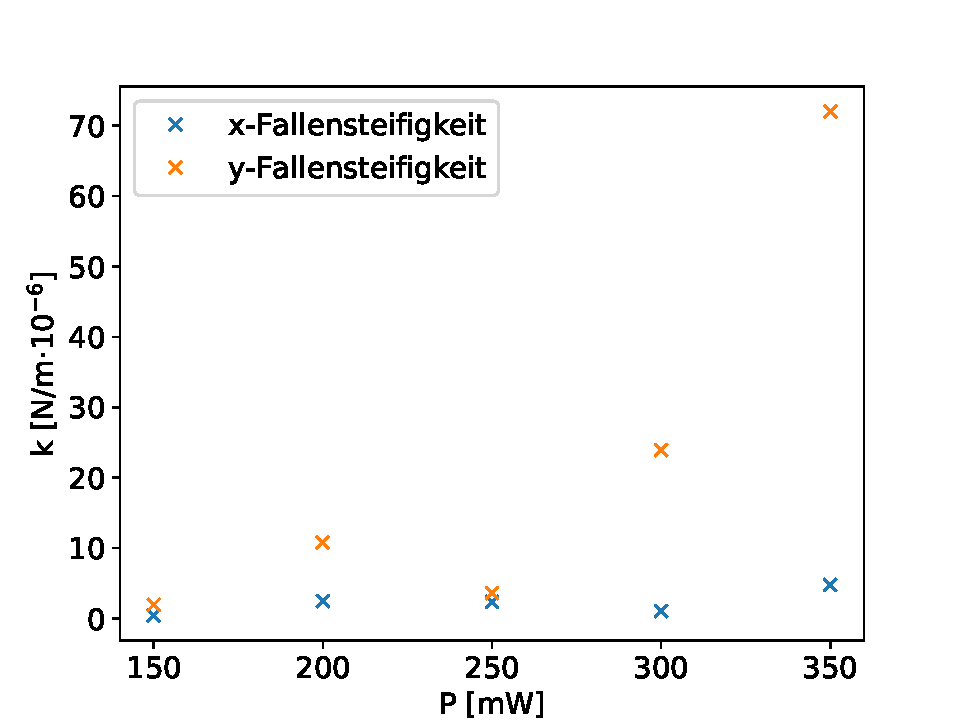
\includegraphics[width = 0.65\textwidth]{k_vortex.pdf}
            \caption{Vom Programm berechnete Fallensteifigkeiten aufgetragen gegen die Laserleistung bei eingesetztem Vortex-Retarder und externer Krafteinwirkung in x-Richtung.}
            \label{fig:k_vortex}
            \end{figure}
            \FloatBarrier
            %
            %
            \begin{table}[h]
                \centering
                \caption{Die vom Programm über die spektralen Leistungsdichten berechneten Fallensteifigkeiten in x- und y-Richtung sowie die daraus berechneten Werte für die Boltzmannkonstante bei verschiedenen Laserleistungen, eingesetztem Vortex-Retarder und externen Krafteinwirkung in x-Richtung.}
                \label{tab:vortex}
                \begin{tabular}{c c c c c}
                \toprule
                {P[mW]} &   {$k_\text{x}$ [N/m $\cdot 10^{-6}$]} & {$k_\text{B,x}$ [J/K]} &{$k_\text{y}$ [N/m $\cdot 10^{-6}$]} & {$k_\text{B,y}$ [J/K]}  \\
                \midrule
                \num{63.4}     &   \num{0.423(20)}	 &  \num{3.93(19)e-24}   &  \num{1.970(20)}     &  \num{8.64(9)e-25}  \\
                \num{93.3}     &   \num{2.470(20)}	 &  \num{8.95(7)e-24}   &  \num{10.800(20)}     &  \num{1.8292(34)e-24}  \\
                \num{123.2}    &   \num{2.400(20)}	 &  \num{8.73(7)e-24}   &  \num{3.610(20)}      &  \num{8.31(5)e-26}  \\
                \num{153.1}    &   \num{1.070(20)}	 &  \num{5.32(10)e-24}   &  \num{23.900(20)}    &  \num{3.6191(30)e-25}  \\
                \num{182.0}    &   \num{4.780(20)}	 &  \num{1.281(5)e-23}   &  \num{72.000(20)}    &  \num{1.18891(33)e-24}  \\
                \bottomrule
                \end{tabular}
            \end{table}
            %

    \newpage
    \subsection{Untersuchung des Vesikeltransports in Zwiebeln}
        \FloatBarrier
        Zur Charakterisierung der Vesikel werden zunächst die Größen der vier in Abbildung \ref{fig:vesikel_size} rot hervorgehobenen Vesikel bestimmt. Dazu wird der Durchmesser der Vesikel über eine 
        Bildbearbeitungssoftware in der Einheit pixel bestimmt und anschließend über die in Abschnitt \ref{sec:Pixel} berechnete Größe eines Pixels im Realraum zu den in Tabelle \ref{tab:d_vesikel} aufgelisteten Werten 
        umgerechnet. Im Mittel ergibt sich so ein Vesikeldurchmesser d$_\text{Vesikel}$ von \SI{0.71(8)}{\micro\metre}.
        %
        \begin{table}[h]
            \centering
            \caption{Die Durchmesser der 4 vermessenen Vesikel in der Einheit von Pixeln und im Realraum}
            \label{tab:d_vesikel}
            \begin{tabular}{c c}
            \toprule
            {d$_\text{Vesikel}$ [Pixel]} & {d$_\text{Vesikel}$ [$\mu$m]}  \\
            \midrule
            $21\pm 4$	 &  $0,67 \pm  0.13$  \\
            $19\pm 4$	 &  $0,60 \pm  0.13$  \\
            $21\pm 4$	 &  $0,67 \pm  0.13$  \\
            $28\pm 4$	 &  $0,89 \pm  0.14$  \\
            \bottomrule
            \end{tabular}
        \end{table}
        %
        \begin{figure}[h]
        \centering
        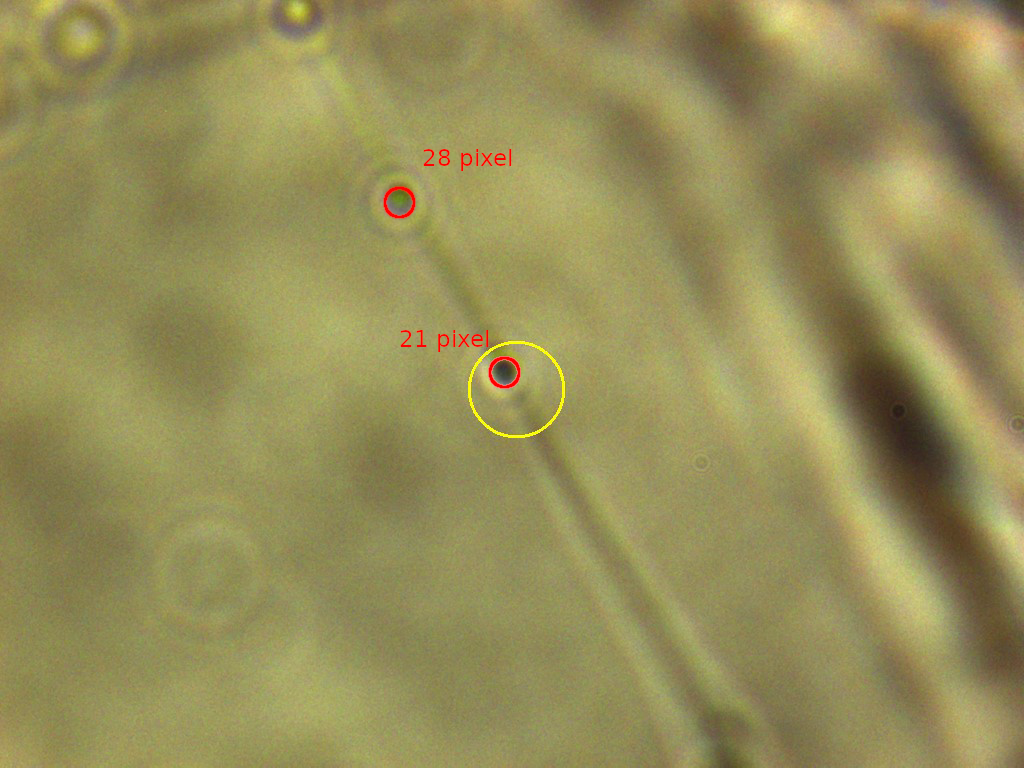
\includegraphics[width = 0.4\textwidth]{pictures/vesikel_size_1.png}
        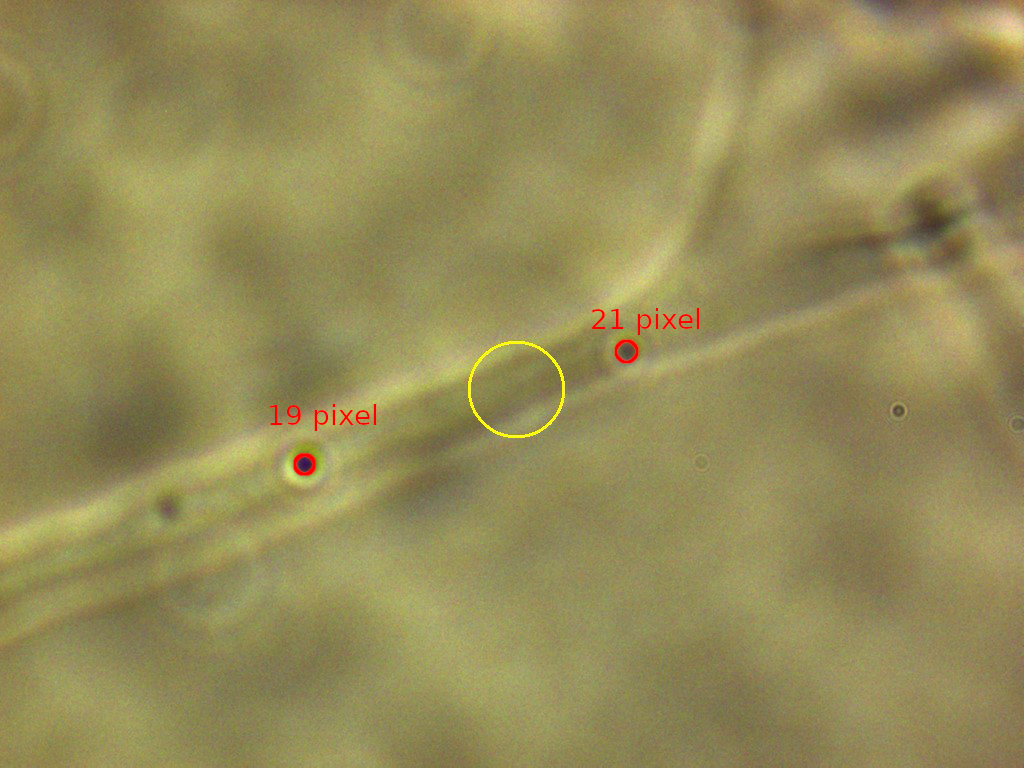
\includegraphics[width = 0.4\textwidth]{pictures/vesikel_size_2.png}
        \caption{Abbildung der vier vermessenen Vesikel, die rot hervorgehoben und deren Größe in Pixeln angegeben sind.}
        \label{fig:vesikel_size}
        \end{figure}

        \FloatBarrier
        %
        \newpage
        Zur Bestimmung der Geschwindigkeit des Vesikeltransports ist die Intensität der Photodiode gegen die Zeit beim Durchlauf eines Vesikels durch die optische Falle in Abbildung 
        \ref{fig:vesikel_size} aufgetragen. Daraus geht eine Durchquerungszeit $\Delta$t von \SI{1}{\second} hervor, die auf eine Vesikelgeschwindigkeit von 
        %
        \begin{equation*}
            v_{\text{Vesikel}} = \frac{2\text{d}_\text{Vesikel}}{\Delta\text{t}} = \SI{1.41(15)}{\micro\metre\per\second}
        \end{equation*}
        %
        schließen lässt.
        %
        \FloatBarrier
        %
        \begin{figure}[h]
        \centering
        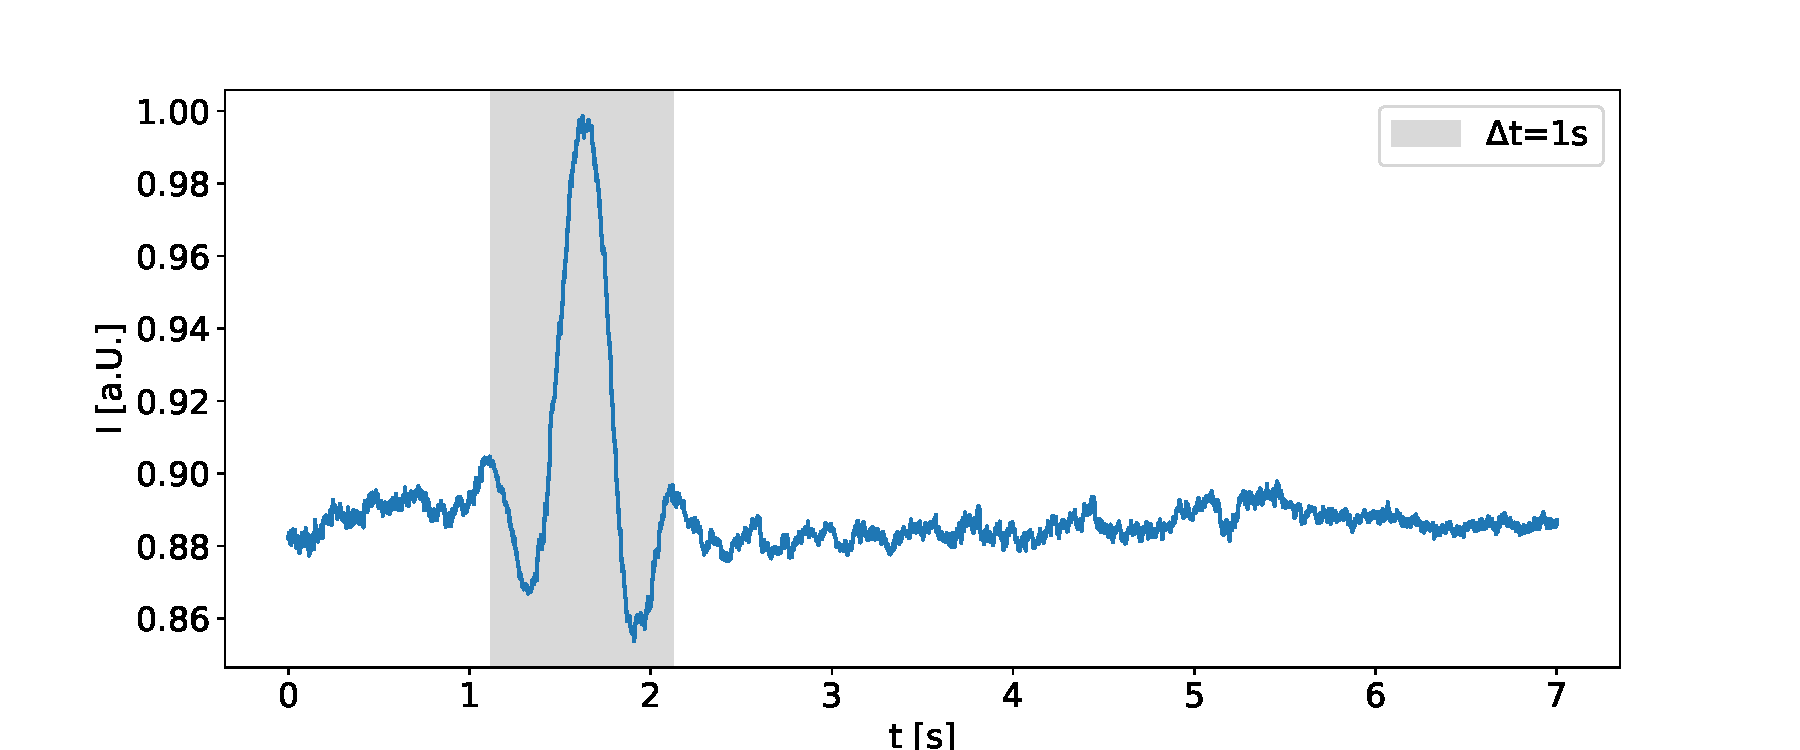
\includegraphics[width = 0.99\textwidth]{v_vesikel.pdf}
        \caption{Auf die Dauer einer Sekunde bestimmte Intensitätsänderung aufgrund des Durchlaufens eines Vesikels durch die optische Falle.}
        \label{fig:v_vesikel}
        \end{figure}
        %
        \FloatBarrier
        %
        \newpage
        Aus den restlichen Videoaufnahmen lassen sich weitere Schlüsse über das typische Verhalten des Vesikeltransports ziehen. So laufen entlang einer Actin-Straße alle Vesikel entlang einer Richtung
        und überholen sich nicht. Wenn ein Vesikel mit Hilfe der optischen Pinzette gegriffen wird, kann es, wie in Abbildung \ref{fig:vesikel_abstand} zu sehen, über \SI{16}{\micro\metre} weit von der 
        Actin-Straße entfernt werden, ohne dass sich die Bindung der Myosin-Motoren zwischen der Straße und dem Vesikel löst. Bei Deaktivieren der optischen Pinzette springt das Vesikel zunächst zurück 
        an seine alte Position und läuft dann weiter in die ursprüngliche Richtung. 
        %
        \FloatBarrier
        %
        \begin{figure}[h]
        \centering
        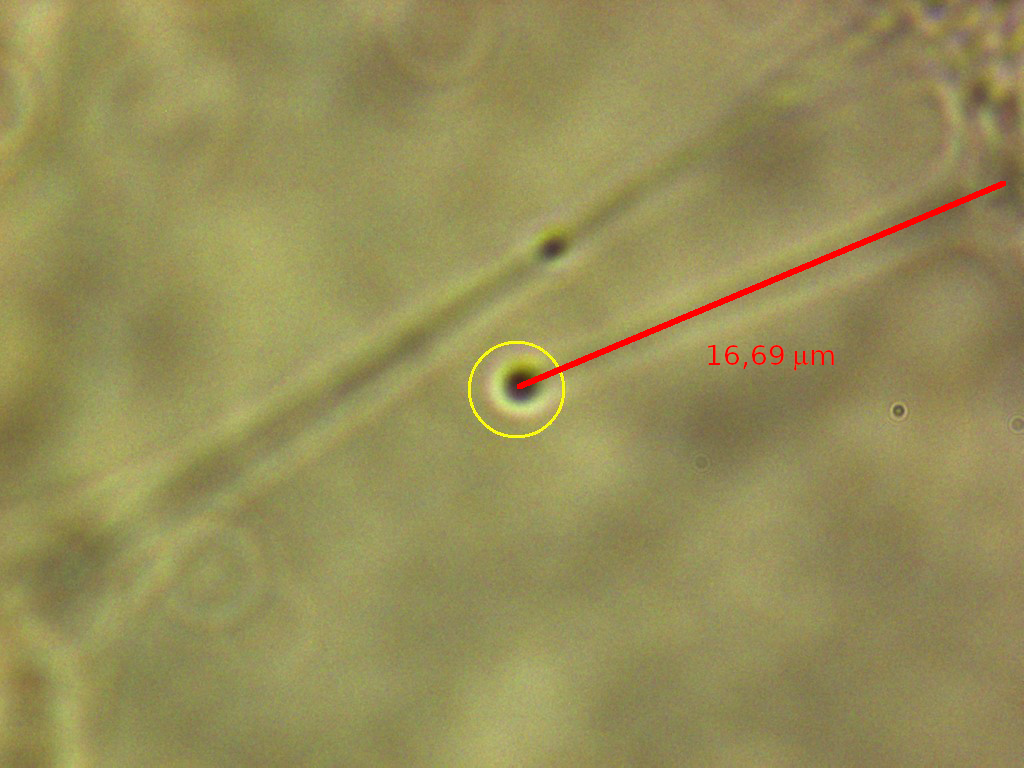
\includegraphics[width = 0.4\textwidth]{pictures/vesikel_abstand.png}
        \caption{Ein Vesikel, das über \SI{16}{\micro\metre} von seiner Ausgangsposition auf der Actin-Straße entfernt wurde.}
        \label{fig:vesikel_abstand}
        \end{figure}
        %
        \FloatBarrier 
        %
        Da die Verbindung der Myosin-Motoren nicht gebrochen werden kann, war es auch nicht möglich Vesikel von einer Straße durch Bereiche ohne Straße auf eine andere zu transferieren. Dies ist in Abbildung
        \ref{fig:vesikel_overlap} zu sehen. Ein Vesikel wird von der Straße am rechten Ende der roten Linie abgefangen und direkt über der blauen Straße platziert. Beim Deaktivieren der optischen Falle geht das 
        Vesikel auf seine Ausgangsposition auf der ehemaligen Straße zurück.
        %
        \FloatBarrier
        %
        \begin{figure}[h]
        \centering
        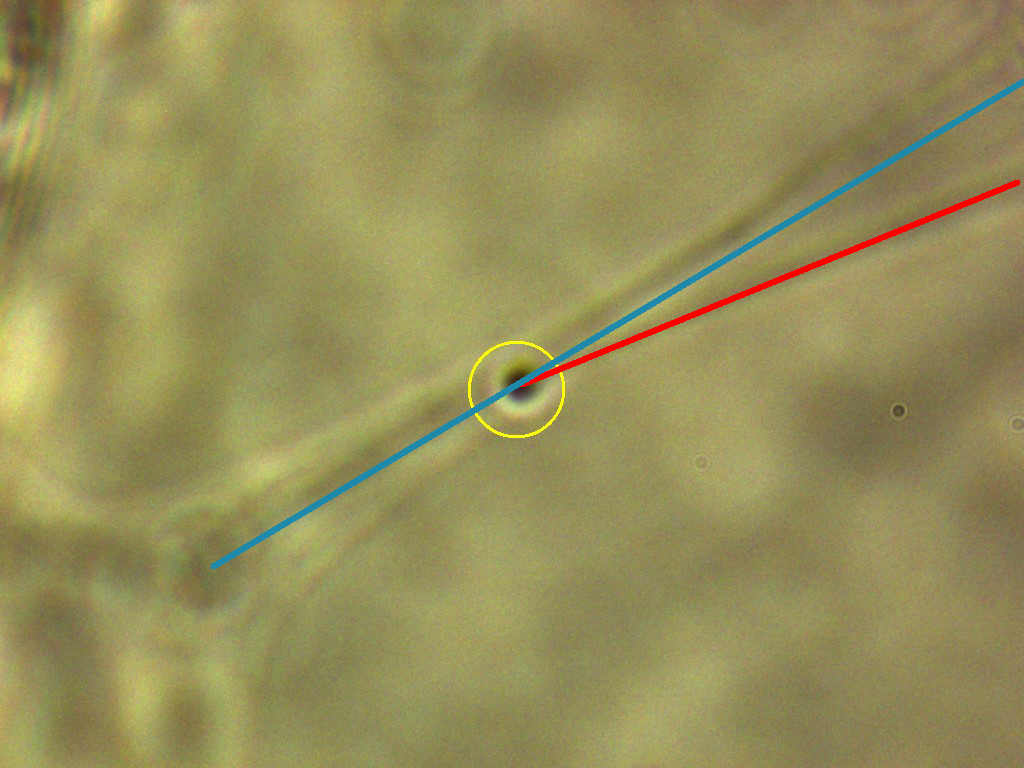
\includegraphics[width = 0.4\textwidth]{pictures/vesikel_overlap.png}
        \caption{Das über der blauen Straße platzierte Vesikel springt bei Deaktivierung der optische Falle auf seine Ausgangsposition auf der Straße am rechten Ende der roten Linie zurück.}
        \label{fig:vesikel_overlap}
        \end{figure}
        %
        \FloatBarrier 
        %
        \newpage
        Auch beim Entfernen der Vesikel von der Straße sind diese jedoch noch beweglich, da die Myosin-Motoren weiterhin funktionieren. In der Nähe einer Kreuzung ist so das schnelle Verschieben der 
        Myosin-Motoren entlang der Kreuzung durch Verschieben des Vesikels, wie in Abbildung \ref{fig:vesikel_sprung} schematisch eingezeichnet, möglich.
        %
        \FloatBarrier
        %
        \begin{figure}[h]
        \centering
        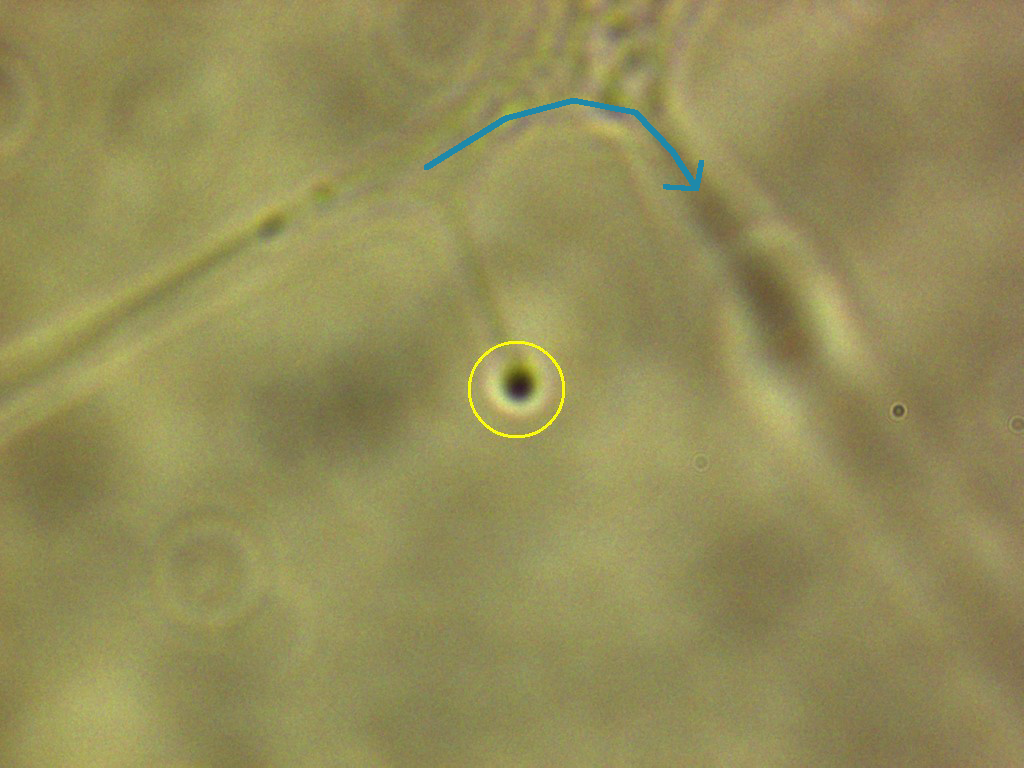
\includegraphics[width = 0.4\textwidth]{pictures/vesikel_transport.png}
        \caption{Bei der gegebenen Vesikelposition können die Myosin-Motoren entlang der Kreuzung auf die andere Straße verfahren.}
        \label{fig:vesikel_sprung}
        \end{figure}
        %
        \FloatBarrier 
        %
        Durch Platzierung der optischen Pinzette über einer Actin-Straße und sukzessivem Erhöhen der Laserleistung ist ein Stopp des Vesikeltransports bei einer Laserleistung bei einer Grenzlaserleistung 
        zu beobachten. Da die zugehörige Aufzeichnung verloren gegangen ist, kann keine genaue Angabe dieser Leistung gemacht werden. Hier wird ein als nicht repräsentativ zu bewertender Erinnerungswert von 
        circa \SI{100}{\milli\watt} genutzt, der einer über die Kalibrierungsmessungen abzuschätzenden Fallensteifigkeit von etwa \SI{2.5e-6}{\newton\per\metre} entspricht. 